\documentclass{article}

% Language setting
\usepackage[english]{babel}

% Set page size and margins
\usepackage[letterpaper,top=2cm,bottom=2cm,left=3cm,right=3cm,marginparwidth=1.75cm]{geometry}

% Useful packages
\usepackage{amsmath}
\usepackage{graphicx}
\usepackage[colorlinks=true, allcolors=blue]{hyperref}

\title{CS461 HW 1}
\author{John Bailon}

\begin{document}
\maketitle

\noindent
Submission Files:

\noindent
John Bailon- CS461 HW1: Homework write up

\noindent
johnbailon-nb-train.py: Code to find densities for Q4.2

\noindent
weights.txt: Mean and variance values used to find densities for Q4.2

\noindent
johnbailon-nb-cls.py: Code for Naive Bayes for Q4.3 and 4.4 

\section{Right Choice for Empirical Metric}

\subsection{Precision Rate}
\[Precision = \frac{True Positive}{True Positive + False Positive}\]

\noindent
If we use precision to measure empirical error, then our model will attempt to minimize the number of False Positives. This will lead to a circle classifier that has a smaller radius and is centered around the largest cluster of positive values.

\begin{figure}[h]
\centering
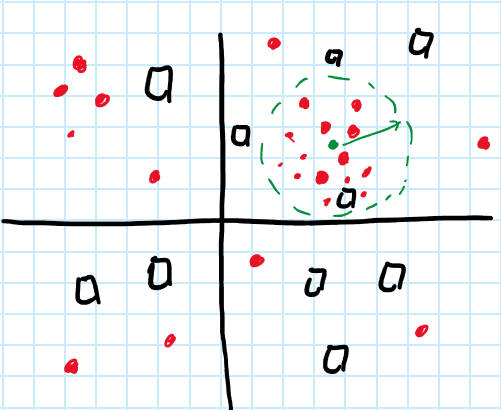
\includegraphics[width=0.35\linewidth]{Precision Figure.png}
\end{figure}

In the above example, the precision rate will minimize the number of false positives. This constricts the circle tightly around the greatest cluster to avoid including negative results within the circle at the expense of missing true positives.

\subsection{Recall Rate}
\[Precision = \frac{True Positive}{True Positive + False Negatives}\]

\noindent
Similar to 1.1, using recall to measure empirical error will lead to us minimizing the number of False Negatives. This will lead to a circle classifier that has a very large radius and is also centered around the largest cluster of positive values.

\begin{figure}[ht]
\centering
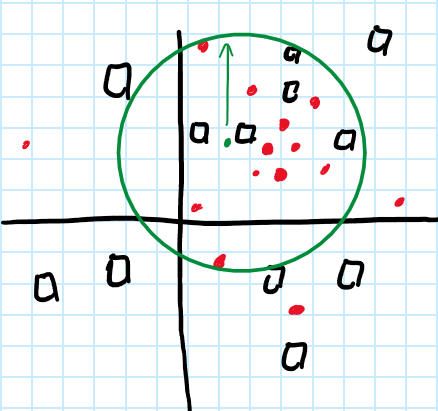
\includegraphics[width=0.35\linewidth]{Recall Figure.png}
\end{figure}

In the example below, we see that the recall rate minimizes false negatives, expanding the radius of the circles to capture as many positives as possible and also capturing negatives in the process.
\newpage
\subsection{Problems with Precision and Recall}
The main problem with precision is that it ignores false negatives, and for recall, it ignores false positives. Precision only looks to minimize false positives and thus constricts the radius smaller to avoid capturing false positives. But this leads to positives that lie outside of the circle. Similarly, recall minimizes false negatives and expands the radius to ensure it captures all positives. But this also captures more negatives in the process.

To avoid these, we can combine precision and recall to balance the weight of false positives and false negatives in our model. Instead, we can minimize a metric like the F1 score, which takes into account both precision and recall.

\[F_1 = 2 * \frac{Precision * Recall}{Precision + Recall}\]

While this won't minimize false positives or false negatives equally, it will create a balance between the two to ensure that we aren't overly restrictive or overly loose in our classifier.

\newpage
\section{Galton Board}

\subsection{Level Sample Spaces}
At each pin, the ball can either move to the left or to the right. At level 2, the ball can fall to the left or the right of the first pin, or left or right of the second pin.

\[\Omega_2 = \{L,R\}\]

\noindent
At level 3, the ball can fall to the left or the right of the first pin, left or right of the second pin, or left or right of the third pin.

\[\Omega_3 = \{L,R\}\]

\noindent
This pattern continues for all \textit{m} levels. At each level, the ball can either move left or right from a given peg.

\[\Omega_m = \{L,R\}\]

\subsection{Sample Space}
The overall sample space $\Omega$ is the Cartesian product of each level in the Galton Board. Each element of the set represents the path to get to the ground level $L_G$. 

\noindent
For example, M=2, the ball can go left or right on the first level peg. Then again left or right on the first peg on the second level, or left or right on the second peg on the second level. The sample space is 

\[\Omega_{M=2} = \{LL\}, \{LR\}, \{RL\}, \{RR\} \]

\noindent
The general form of this is the combination of all L, R choices M times.
\[\Omega = \{L_1, L_2, L_3, \dots,L_m : L_i \in \{L,R\}, \forall i = 1, 2, 3, \dots, M\}\]

\subsection{Meaning of the End Position L}

The location $L_G$ is the endpoint of any given path from the start of the Galton Board. We can look one level ahead to see that reaching a bottom position stems from the left or right choice from the peg in level M-1. Similarly, to get to those pegs, it stems from left or right choices from the above peg in M-2. We can think of any position at the bottom as the difference between the sum of left choices and the sum of right choices made while traversing the galton board

\subsection{Random Variable Mapping}

We can represent the decision to move left or right numerically. If the ball moves right, we'll represent that with a 1, and if it moves left, a 0. 

 \[ I = \begin{cases} 
     $0$ \text{   if left}\\
     $1$ \text{   if right}
   \end{cases}
\]

$L_G$ then is the sum of all these moves taken at each level to get to the given end position. Let X be the random variable, which is the sum of moves from the path to get to a given endpoint.

\[X_i = \sum^{M}_{i = 1} I\]

\subsection{Probability Mass Function and Central Limit Theorem}

Since we are counting the number of right turns made at each peg, we can represent the PMF for X as a binomial distribution. 

\[P(X = right) = {M \choose x} (0.5)^M\]

Where M is the depth of the galton board and x is the number of right turns made in the path.

Various depths are listed below

\[P(X = right) = {5 \choose x} (0.5)^5\]
\[P(X = right) = {10 \choose x} (0.5)^{10}\]
\[P(X = right) = {100 \choose x} (0.5)^{100}\]

\begin{figure}[h]
\centering
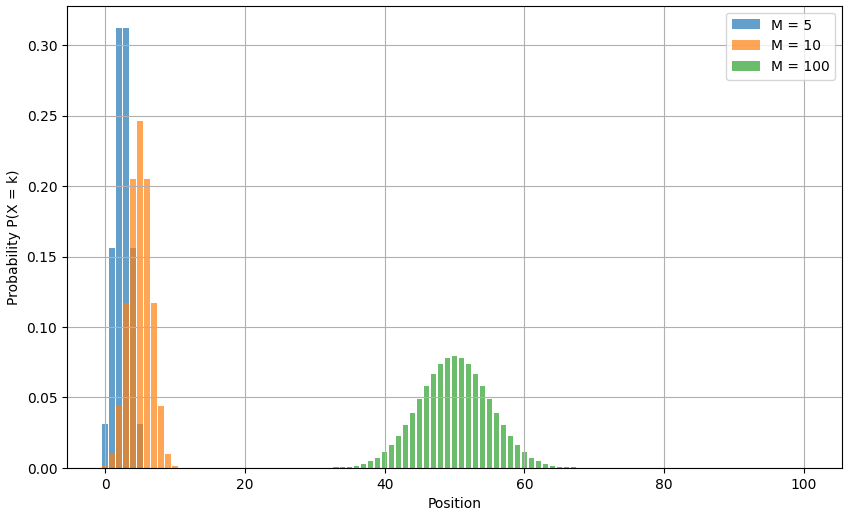
\includegraphics[width=0.80\linewidth]{2.5 Graph.png}
\end{figure}

As M increases, the distribution resembles a bell curve more and is shifted to the right. We assume that each decision at each peg is independent from each other. As we add more depth, the standard deviation of the sum grows by the square root of the number of trials. This tightens the distribution around the mean, resulting in a bell shape as we make M very large.

\newpage
\section{Bayes Rule}

From the problem statement, some probabilities are directly given. We know that the plant has a 20\% chance to die if properly watered and an 80\% chance to die if improperly watered. The probability our friend will forget to water the plant is 30\%.

\[P(Die | Water) = 0.7\]
\[P(Die | \neg Water) = 0.3\]
\[P(Water) = 0.7\]
\[P(\neg Water) = 1 - P(Water) = 0.3\]

\subsection{Plant Survival}
The probability that our plant will survive at the end of the week can be derived using the law of total probability. We sum up the chance the plant survives given that our friend watered it, and if our friend doesn't water it

\[P(\neg Die) = 1 - ( P(Die | Water) * P(Water) + P(Die | \neg Water) * P(\neg Water) ) \]
\[P(\neg Die) = 1 - (0.2*0.7) + (0.8*0.3) = 0.62 \]

\noindent
Our plant has a 62\% chance of surviving the week.

\subsection{Friend Forgets to Water}
Put another way, this question asks what is the chance the plant is dead given our friend  This probability was described in the problem statement.

\[P(Die | \neg Water) = 0.3\]

\subsection{Dead Plant, Forgetful Friend?}
This question asks the opposite of 3.2. It asks what the chance is that our friend forgot to water the plant, given that it is dead. We can derive this using Bayes Rule.

\[P(\neg Water | Die) = \frac{P(Die | \neg Water) * P(\neg Water)}{P(Die)} = \frac{(0.8*0.3)}{(1-0.62)} = 0.63\]

Given that our plant is dead, the chance our friend forgot to water it is 63\%.

\newpage
\section{Naive Bayes}

\subsection{Model Equation}
We know that glucose and blood pressure are conditionally independent given D+, so we can separate each factor and multiply them together.

\[P[D=+ |G =g, B=b] = \frac{P[G=g,B=b|D=+] * P[D=+]}{P[G=g, B=b]} \]
\[P[D=+ |G =g, B=b] = \frac{P[G=g|D=+] * P[B=b|D=+] * P[D=+]}{P[G=g, B=b]} \]

Similarly, for D - 
\[P[D=- |G =g, B=b] = \frac{P[G=g|D=-] * P[B=b|D=-] * P[D=-]}{P[G=g, B=b]} \]

To implement Naive Bayes, we will calculate these probabilities and assign a prediction based on the highest probability. Since the denominator is constant in both probabilities, we can ignore this in our calculations.

We will compare the following probabilities for each given record and return the greater probability. 1 for a positive diabetes prediction and 0 for a negative prediction 
\[P[D=+ |G =g, B=b] \propto P[G=g|D=+] * P[B=b|D=+] * P[D=+] \]
\[P[D=- |G =g, B=b] \propto P[G=g|D=-] * P[B=b|D=-] * P[D=-] \]

\subsection{Training Densities}
Code for training is found in the submission as johnbailon-nb-train.py. To find these densities, I converted the train.csv into a pandas data frame. I split them into positive diabetes and negative diabetes, and for each, I found the mean and variance for each bp and glucose.
Weights were saved to weights.txt and are listed below, rounded to 3 dp

\[f_G(g | D+) = N(44.633, 81.360)\]
\[f_G(g | D-) = N(44.143, 13.430)\]
\[f_G(bp | D+) = N(71.628, 40.861) \]
\[f_G(bp | D-) = N(86.793, 21.190)\]

Priors were also found based on the training data
\[P(D+) = 0.511\]
\[P(D-) = 0.489\]

\subsection{Naive Bayes Code}
Code for Naive Bayes is found in the submission as johnbailon-nb-cls.py. 

\subsection{Evaluating the Model}
Code for Naive Bayes is found in the submission as johnbailon-nb-cls.py. Evaluating my model using the test data set, my model has a 92.31\% accuracy.

\subsection{Standardization}
 Generally speaking, it is best practice to standardize data as different data points may have different magnitudes, affecting model performance. It is important to standardize the data by looking at distributions rather than the absolute range. For example, if we were to build a model to predict house prices by looking at the area in sq feet and the number of bathrooms, the magnitude of the area would be much greater than the number of bathrooms. 

 In this specific case, I did not standardize my data. The normal range of blood pressure and glucose readings are relatively similar in magnitude. This means the magnitude of each point of data won't affect the model in a significant way.
 

\subsection{Model Reflection}
The data doesn't reflect reality well. Assuming that glucose is measured in mg/dL, many of the data points in the training set range from 35-40 mg/dL, well below normal levels, and is an indicator of severe hypoglycemia, which is life-threatening. The sample also doesn't reflect the population well. In the test set, almost 51\% of the data points had diabetes, well above the current estimate in the US, which is around 11\%  

To improve the data, we can use various pre-processing techniques to minimize noise by implementing PCA or whitening. PCA might not be the best choice since our data has low dimensionality, but whitening helps standardize the data. 

\newpage
\section{Data Whitening}

\subsection{Expressions}
\subsection{Whitening}

\newpage
\section{ML and MAP Estimation}

\subsection{}
\subsection{}
\subsection{}

\end{document}